\section{Inleiding}

Nu machine learning steeds meer toepassingen krijgt, gaat men ook veel meer machine learning modellen gebruiken in de productieomgeving.
Traditioneel werden deze modellen toegepast op centrale servers of gedistribueerde cloud servers. Hierdoor moet er een grote hoeveelheid data verstuurd worden over het internet.
Dit is echter niet zo schaalbaar als men op grote schaal met heel veel verschillende kleine toestellen, data gaat opmeten. % TODO: Waarom niet schaalbaar?

\begin{figure}[ht]
	\centering
	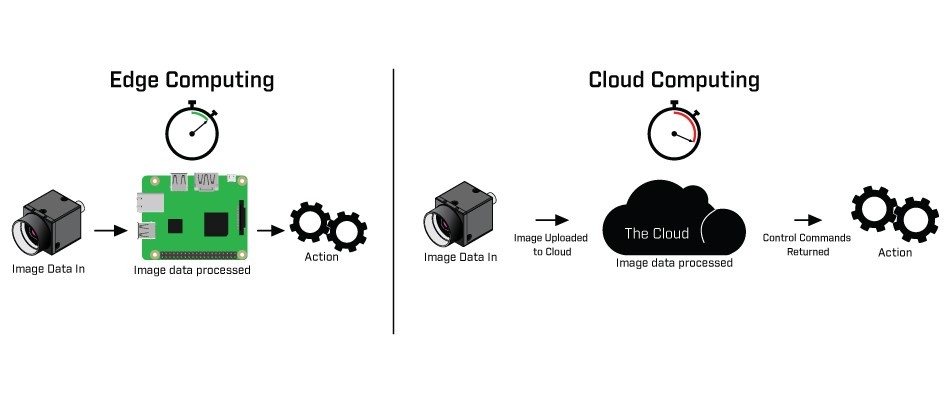
\includegraphics[width=0.9\textwidth]{figuren/iisedgecomputing.jpg}
	\caption{Edge vs. Cloud computing}
	\cite{flir-edge-computing}
	\label{fig:edge-vs-cloud}
  \end{figure}


Er is gelukkig een grote 'paradigm shift' aan de gang waarbij men meer en meer machine learning gaat uitvoeren in embedded devices.
Dit is mogelijk omdat deze embedded devices steeds sneller en beter worden in het verwerken van data.
Op deze manier kunnen wij het machine learning model dichter bij de sensor plaatsen. Zo minimaliseren wij het benodigde netwerkverkeer.
Ook de latency of vertraging tussen opname en actie is veel kleiner. \cite{flir-edge-computing}

De ruwe data van de sensoren kan soms ook sensitieve informatie bevatten zoals gezichten of nummerplaten. Omdat we deze on-edge verwerken hoeven deze niet naar de cloud gestuurd te worden waar ze onderweg misschien onderschept kunnen worden \cite{flir-edge-computing}.

Het is echter niet zo simpel om de code geoptimaliseerd voor multi-core servers zomaar over te zetten naar de kleine, vaak single-core, microprocessors van deze embedded devices. In dit verslag leg ik het proces een beetje uit om een Convolutional Neural Netwerk (CNN) in python code, over te zetten naar C code voor op de 32-bit ARM Cortex M-7.

\section{Feature extraction}

\section{Convolutional Neural Network (CNN)}

\subsection{Structuur van ons CNN-model}

\subsection{Training}
\subsubsection{Resultaten}


\section{Edge implementatie}

\subsection{Kwantisatie van ons CNN-model}
\subsubsection{Qm.f formaat}

\subsection{Experiment met microfoon}
\subsubsection{Resultaten}


\section{Conclusie}